%!TEX root = ../dissertation.tex
\begin{savequote}[0.6\textwidth]
	\itshape In the beginning, there was nothing. \\
	\itshape And God said, Let there be light. \\
	\itshape And there was light. \\
	\itshape There was still nothing, \\
	\itshape but you could see it a lot better.
	\qauthor{---Woody Allen}
\end{savequote}

\chapter{GaudiMM}
\label{chap:04}

% \section{Introduction $\&$  motivation}
% \addcontentsline{toc}{section}{Introduction $\&$  motivation}

\todo[inline]{See nueva-gaudi}

\todo[inline]{Modular nature of the tool}

Before introducing all its features and capabilities, it will be convenient to review \todo{multiobjective} optimization techniques and how they are applied routinely in computational chemistry and molecular modeling. That way, it will be easier to grasp the rationale behind the terminology used in some of its key concepts.

\section{Rationale behind the idea}

%%%%%%%%%%%%%%%%%%%% Table No: 1 starts here %%%%%%%%%%%%%%%%%%%%


\begin{table}[hbtp]
	\caption{GaudiMM: technical datasheet}
	\footnotesize
	\newcolumntype{R}{>{\hsize=.25\hsize\raggedleft\arraybackslash}X}%
	\newcolumntype{L}{>{\hsize=.75\hsize\raggedright\arraybackslash}X}%
	\newcommand{\tableheading}[1]{\multicolumn{2}{c}{\textsc{#1}}}
	\begin{tabularx}{\textwidth}{RL}
		\toprule
		%row no:1
		\tableheading{GaudiMM} \\
		\toprule
		%row no:2
		\textit{Description} & A modular optimization platform for molecular design \\
		\midrule
		%row no:3
		\textit{Requirements} & Python, UCSF Chimera, OpenMM, IMP, DSX, ProDy... \\
		\midrule
		%row no:4
		\textit{License} & Apache 2 \\
		\midrule
		%row no:5
		\textit{Download} & \href{https://github.com/insilichem/gaudi}{github.com/insilichem/gaudi} \\
		\midrule
		%row no:6
		\textit{Documentation} & \href{https://gaudi.readthedocs.io}{gaudi.readthedocs.io} \\
		\midrule
		%row no:7
		\textit{Citation} & J. Comput. Chem. 2017, 38, pp 2118–2126. DOI: 10.1002/jcc.24847 \\
		\bottomrule

	\end{tabularx}
\end{table}


%%%%%%%%%%%%%%%%%%%% Table No: 1 ends here %%%%%%%%%%%%%%%%%%%%



GaudiMM is a Python package that allows to build and refine of chemobiological structures through multi-objective optimization. Built on top of the NSGA-II algorithm, it features a modular, extensible architecture that conceptually emphasizes the three main stages of the optimization process: exploration, evaluation and selection. This section will describe all the details behind its rationale and implementation in a molecular modeling environment. For practical use cases, please refer to \autoref{chap:06}, where several examples are presented.

\section{Implementation}

\todo[inline]{Complete this section}

\begin{itemize}
	\item Draft \& sketch molecules
	\item Give answers to quick hypotheses
	\item Worry about fine details later - starting points do not need them
\end{itemize}

\subsection{The NSGA-II algorithm}
% \addcontentsline{toc}{subsection}{The NSGA-II algorithm}
NSGA-II is a multi-objective genetic algorithm (MOGA) developed by K. Deb. It has been thoroughly tested and benchmarked in well-characterized multi-objective problems\cite{nsgaii} and is considered a prototypical MOGA.

The algorithm can be described in three main stages (exploration, evaluation and selection) that are executed iteratively until an exit condition is met (usually, convergence or maximum steps). Generating new candidate solutions or individuals is considered within the \textit{exploration} stage, and can be achieved by random attribute generation or combining previously existing individuals. In the evaluation stage, the candidates are assessed with different functions or objectives, each returning a scalar that represents a fitness score for that objective. Finally, the selection stage collects all the individuals and compares their scores to select the best individuals according to the Pareto dominance criterion.

In more detail, NSGA-II starts with the generation of a random set of potential solutions (\textit{individuals}) which comprise the so-called \textit{initial population}. This first set of individuals is then evaluated with one or more \textit{cost functions} and each individual is assigned a \textit{fitness }score vector, the elements of which are the result of those cost functions. At this point, a small subset of the population is submitted to a round of random modification of parameters (mutation) or exchanging some of their attributes (recombination), and are then assessed by the same cost functions. Being random, the results of these variations can be better or worse than their preceding counterparts (parents). Finally, both the offspring and the parental generation ($ \mu $ +$ \lambda $  strategy) compete in the selection tournament, which will rule which ones will replace the initial population. After a number of iterations, the initial population will have evolved and, eventually, will end up providing reasonable solutions to the problem that represent a compromise between the analyzed variables (see fig. \ref{fig:nsga}).




\begin{figure} % FIXME!
	\vspace*{-1cm}
	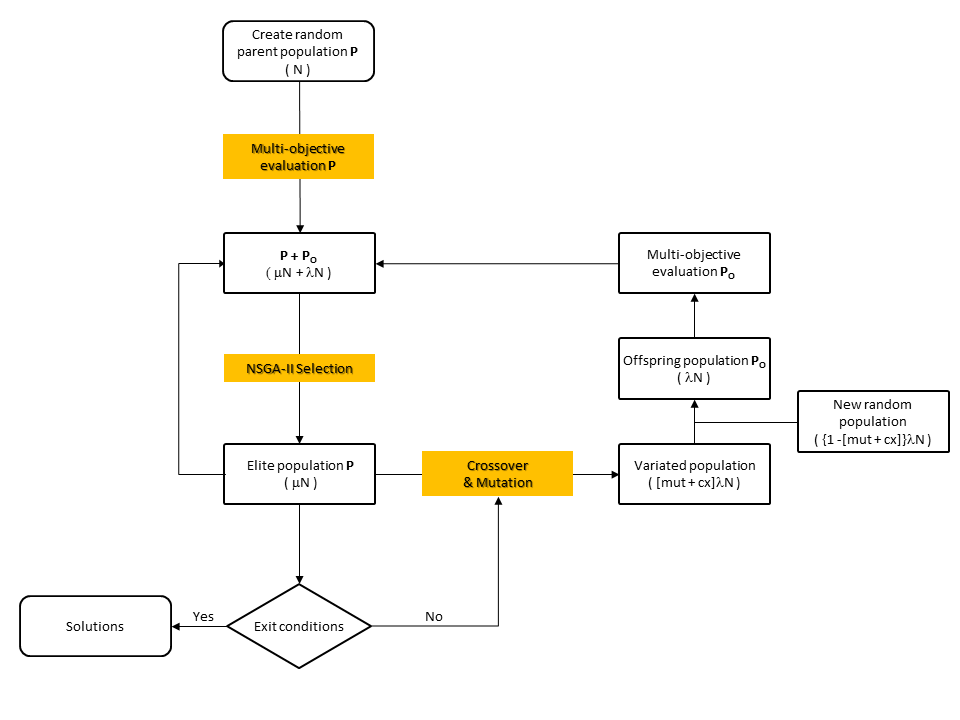
\includegraphics[width=0.9\textheight,angle=90]{./figures/04/nsga.png}
	\cprotect\caption[NSGA-II algorithm]{Flowchart of the modular NSGA-II multi-objective genetic algorithm (MOGA) implemented in GaudiMM. $ N $ is the number of individuals in the initial population $P$. Values $\lambda$ and $\mu$ are related to the number of children produced at each generation and the number of individuals selected for the next generation, respectively. Together they control the offspring population size, $ P_{0} $. Constants $ mut $ and $ cx $ are the probabilities associated to mutation and crossover.}
	\label{fig:nsga}
\end{figure}


\subsection{Of individuals and genes: the exploration stage}
% \addcontentsline{toc}{subsection}{Of individuals and genes: the exploration stage}
The initial step of all the iterations in the algorithm is the exploration, which is responsible for the generation of new candidate solutions. A candidate solution is defined by a list of attributes, each representing the state of a molecular property. Generating new solutions simply involves changing the value of one or more attributes in that list.

Since GaudiMM is based on a genetic algorithm, the implementation follows the same biologicist terminology. In GaudiMM any candidate solution is encoded in a special object called \textit{Individual}. All \textit{Individual} objects in the simulation are defined by the same high-level attributes, which are called \textit{genes}. In the same fashion, the state of each gene is defined by its \textit{allele} attribute. Depending on the gene, the allele can be a list of numbers, a path to a file, a matrix$ \ldots $

For example, a typical optimization problem is finding the dihedral torsion that gives the minimum energy in the ethane molecule. The Individuals featured in this example would only need exploring a single variable, the torsion angle of the C-C bond, with values ranging from 0 to 360º. In GaudiMM-speak, the gene would be the bond \textit{rotator} and the allele the different angles.

The key part of genetic algorithms is the implementation of variation operators as part of the exploration stage. Instead of merely trusting randomness, existing solutions are combined in hopes of obtaining a better child solution. These two operations are called mutation and crossover or mating, mimicking what happens in the cell nucleus at the chromosomic level.





\begin{figure}[H] % FIXME!
	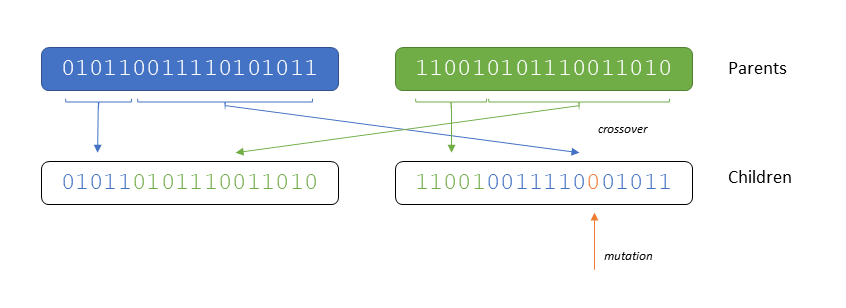
\includegraphics[width=\textwidth]{./figures/04/ga-crossover-mut.png}
	\caption[Mutation and crossover]{Mutation and crossover operations introduce variability in the parental population.}
	\label{fig:cxmut}
\end{figure}



Taking all these requirements into account, genes in GaudiMM are programmatically defined by four functions (express, unexpress, mutate and mate) and an attribute (allele). Additional methods and attributes can be defined to support these required elements, if needed. Since each gene is a clearly separate entity, the Individual object can feature more than one gene, and one gene can be present more than once with different parameters.

This adds an unprecedented versatility when configuring a GaudiMM calculation: the user can decide which molecular features must be assessed for every case. For conformational searches it might be enough with the Torsion gene, but for protein-ligand docking the Search gene will be required too. Additionally, if the built-in genes do not fulfill the requirements of the simulation, new ones can be written and added to GaudiMM thanks to is modular architecture and well-defined programmatic interface.

This is, genes are more than simple \textit{allele} attribute holders: they are high-level abstractions of operators that can make reversible changes in a molecule based on the value of its allele. Like in Biology, changes in the allele are only visible if the corresponding gene is being \textit{expressed}. In those terms, GaudiMM genes encompass both the allele and the expression mechanism. In the previous example, when the allele changes the torsion gene needs to update the coordinates of the atoms affected by the dihedral rotation, and only those. To make changes consistent, it might also need to \textit{unexpress} or undo those changes to the original state. These changes can happen in the topology or in the coordinates of an associated molecule.

\subsubsection{Topology modifiers}
% \addcontentsline{toc}{subsubsection}{Topology modifiers}
Genes that fall in this category perform modifications on the atoms that conform the molecular structure and/or their connectivity. For example, they could increase the length of a ligand linker, change the metal element of a metallic cofactor or mutate some residues in a peptide sequence.

\begin{itemize}
	\item \textsc{Molecule}. It is the main gene, as it will be used to load molecular structures from files (PDB, mol2, xyz or anything else supported by UCSF Chimera). All other genes depend on the initial topology and coordinates provided by one or more Molecule genes. In addition to loading files, the `path` parameter support loading from a directory, whose contents determine the final behavior:
	\begin{itemize}
		\item If the directory contains molecule files, the allele will be set to one of them randomly for each individual. This allows GaudiMM to deal test a library of compounds against certain criteria; i.e. virtual screening.
		\item If the directory contains subdirectories which, in turn, contain molecules files, the gene will sort those subdirectories by name and then pick one molecule from each, in that order. The chosen molecules will constitute the allele and will be chained linearly as specified in the accompanying meta file, which lists the serial number of the potential donor and acceptor atoms.
	\end{itemize}
	\item \textsc{Mutamers}. Given a residue position in a protein structure, it can replace its sidechain to any other natural amino acid specified in the configuration. Useful to study site mutations.
\end{itemize}

\subsubsection{Coordinates modifiers}
% \addcontentsline{toc}{subsubsection}{Coordinates modifiers}
Genes that fall in this category only alter the positions of the atoms involved in a molecular structure. They can modify the full structure, like a rigid translation or rotation of the molecule, or only a part, like the sidechain orientation of a protein residue.

\begin{itemize}
	\item \textsc{Torsion}. It helps explore small molecules flexibility by performing bond rotations in the selected Molecule objects, if they exhibit free bond rotations.

	\item \textsc{Search}. It performs rigid transformations on Molecules (translation and rotation). A radius parameter can be set to limit the search sphere range. If the radius is zero, the molecule won’t be translated but can freely rotate around the anchor atom, which is useful for covalent bond emulation.

	\item \textsc{Rotamers}. It allows to explore side-chain conformations in protein residues by applying Dunbrack’s\cite{dunbrack1993backbone} or Dynameomics\cite{scouras2011dynameomics} rotamer libraries.

	\item \textsc{NormalModes}. Given a Molecule object, it calculates normal modes with elastic network methods and applies the resulting collective motions as possible variants of the initial coordinates set.

	\item \textsc{Trajectory}. Given a molecular dynamics trajectory file, it can retrieve random frames and apply the resulting coordinates to any Molecule object.
\end{itemize}


\begin{table}[hbtp]
	\caption[List of genes implemented in GaudiMM]{List of genes implemented in GaudiMM.}
	\label{table:gaudi-genes}
\footnotesize
\newcolumntype{L}{>{\hsize=.25\hsize\raggedright\arraybackslash}X}%
\newcolumntype{M}{>{\hsize=.5\hsize\raggedright\arraybackslash}X}%
\newcolumntype{R}{>{\hsize=.25\hsize\raggedright\arraybackslash}X}%
\begin{tabularx}{\textwidth}{LMR}
%row no:2
\toprule
\textsc{Name} & \textsc{Description} & \textsc{Depends on} \\
\toprule
%row no:3
 Molecule & Load and build structures & UCSF Chimera \\
\hhline{~~~}
%row no:4
 Rotamers & Explore side chain flexibility & UCSF Chimera \\
\hhline{~~~}
%row no:5
 Mutamers & Explore mutation of residues & UCSF Chimera \\
\hhline{~~~}
%row no:6
 NormalModes & Explore collective motions & ProDy \\
\hhline{~~~}
%row no:7
 Search & Translation and rotation of Molecules & UCSF Chimera \\
\hhline{~~~}
%row no:8
 Torsion & Dihedral rotation of bonds & UCSF Chimera \\
\hhline{~~~}
%row no:9
 Trajectory & Load frames from MD trajectories & MDTraj \\
\bottomrule
\end{tabularx}
\end{table}


%%%%%%%%%%%%%%%%%%%% Table No: 2 ends here %%%%%%%%%%%%%%%%%%%%



\subsection{Of environments and objectives: the evaluation stage}
% \addcontentsline{toc}{subsection}{Of environments and objectives: the evaluation stage}
After generating candidate solutions, these must be evaluated with the optimization criteria. In genetic algorithms, this is usually called assessing the fitness of the individuals: fitter individuals are more qualified to survive in the environment.

Mimicking these concepts, the GaudiMM implementation creates an Environment object that list the optimization criteria, each represented by an Objective entity. Objectives are also independent units that can be instantiated multiple times in the same Environment, but the defined interface is simpler that in genes: a ‘weight’ attribute defines the optimization type (maximization or minimization), and a function named ‘\textit{evaluate’} that takes an Individual object and returns a numerical value as result. What the \textit{evaluate} function does behind the scenes does not actually matters as long as a number is produced: calculate a distance between two atoms, retrieve a parameter from a database, compute the potential energy with an external MM library$ \ldots $

As a result, GaudiMM ships with a rather diverse set of objectives, combining 3\textsuperscript{rd} party packages and custom developments in the same distribution. Together they cover all kinds of energetic, geometric and spatial measurements, allowing to use different levels of theory at the same time in a seamless workflow. Any geometric or energetic parameters that could describe a molecular system can be used as objectives to drive the GA exploration. This allows us to turn the tables on routine protocols based on computing energetic optimizations and then analyzing the results in hopes of finding a suitable model that fits the intended restraints; i.e. those same analysis tools can guide the optimization process from the beginning.

\subsubsection{Geometry measurement}
% \addcontentsline{toc}{subsubsection}{Geometry measurement}
\begin{itemize}
	\item \textsc{Angle}. Given three atoms, this objective calculates the angle between those. By minimizing the difference between the measured angle and the target one, the final angle can be optimized. It will calculate the dihedral if four atoms are specified.

	\item \textsc{Distance}. If two atoms are provided, this objective calculates the distance between. By minimizing the difference against a target value, the structure can be optimized to fulfill that requirement. It also supports calculating distances to groups of atoms by taking the centroid of the group.

	\item \textsc{Inertia}. This objective calculates the inertia tensors of two structures and returns the sine of the smallest angle formed between any of the possible pairings. It can be useful to align ligands along the major axis of a protein.


\end{itemize}\subsubsection{Spatial measurement}
% \addcontentsline{toc}{subsubsection}{Spatial measurement}
\begin{itemize}
	\item \textsc{Solvation}. Solvent-Accessible Surface Area (SASA) and Solvent-Excluded Surface Area (SESA) are two common techniques to describe the solvation of a structure. It can be used to optimize structures in terms of exposure of inside pockets or their folding. By maximizing SASA or SESA, the structure will tend to open up; by minimizing those values, the trend will be towards a more compact conformation.

	\item \textsc{Volume}. This objective calculates the volume occupied by a structure. It does so by computing the solvent-exposed surface of the structure, which is then considered as a polyhedron of thousands of triangular faces.


\end{itemize}\subsubsection{Energy calculation}
% \addcontentsline{toc}{subsubsection}{Energy calculation}
\begin{itemize}
	\item \textsc{DSX}. DrugScoreX is a knowledge-based docking scoring function developed by Neudert $\&$  Klebe.\cite{neudert2011dsx} It is specially designed to compute interaction energies between protein structures and small compounds. This objective is a Python wrapper around the DSX executables and input files.

	\item \textsc{Energy}. This objective allows to calculate the potential energy of a structure with the Molecular Mechanics force fields implemented in OpenMM. Parameters must be provided for custom residues.

	\item \textsc{LigScore}. Another docking scoring function developed by Sali\cite{krammer2005ligscore} which allows to obtain protein-ligand interaction energies. While the parent project, IMP,\cite{russel2012putting} is a C++ project with Python bindings, the LigScore function is only exposed through an executable. This objective can call that binary and parse the resulting energies from the output.

	\item \textsc{Vina}. AutoDock Vina\cite{trott2010autodock} is a popular open-source package to perform protein-ligand docking. This objective calls the Vina executable in score-only mode to calculate the interaction energies between a protein and a ligand.

	\item \textsc{GOLD}. This commercial software suite is one the most used solutions to calculate accurate docking poses. With this objective, all the scoring functions exposed in GOLD\cite{gold} can be used as guiding evaluators in GaudiMM: PLP, GoldScore, ChemScore$ \ldots $  License is needed for this to work.

	\item \textsc{NWChem}. This objective provides a way to run quantum mechanics calculations in this popular open-source software suite.\cite{nwchem} Provided a template input-file, this objective will insert the appropriate coordinates, charge and multiplicity. While all methods implemented in NWChem are potentially usable, only semi-empirical ones are recommended in terms of speed; specially for large structures.


\end{itemize}\subsubsection{High-level chemical descriptors}
% \addcontentsline{toc}{subsubsection}{High-level chemical descriptors}
\begin{itemize}
	\item \textsc{Contacts}. This objective can calculate two type of distance-based energy descriptors. When the ‘hydrophobic’ mode is chosen, this objective will maximize potentially attracting interactions between close enough atoms by applying a Lennard-Jones-like scoring function. If the ‘clashes’ mode is chosen, it will minimize the steric hindrance of the structure by minimizing the volumetric overlap of the Van der Waals spheres of atoms that are too close.

	\item \textsc{HBonds}. This objective uses geometrical criteria to calculate the number of hydrogen bonds between potential donors and acceptors.

	\item \textsc{Coordination}. By applying a type of computer vision algorithm called Point Set Registration, this objective can identify potential coordination geometries around a metal center. It returns the RMSD similarity between the first coordination sphere and the ideal polyhedron: the lower the value, the better the geometry.
\end{itemize}


\begin{table}[hbtp]
	\caption[List of objectives implemented in GaudiMM]{List of objectives implemented in GaudiMM.}
	\label{table:gaudi-objectives}
\footnotesize
\newcolumntype{L}{>{\hsize=.15\hsize\raggedright\arraybackslash}X}%
\newcolumntype{M}{>{\hsize=.65\hsize\raggedright\arraybackslash}X}%
\newcolumntype{R}{>{\hsize=.20\hsize\raggedright\arraybackslash}X}%
\begin{tabularx}{\textwidth}{LMR}
\toprule
\textsc{Name} & \textsc{Description} & \textsc{Depends on} \\
\toprule
%row no:3
 Angle & Optimize angle of three atoms, or dihedral of four atoms & UCSF Chimera \\
\hhline{~~~}
%row no:4
 Contacts & Minimize steric clashes, maximize hydrophobic interactions & UCSF Chimera \\
\hhline{~~~}
%row no:5
 Coordination & Optimize coordination geometry of metal center & In-house \\
\hhline{~~~}
%row no:6
 Distance & Optimize distance between two or more atoms & UCSF Chimera \\
\hhline{~~~}
%row no:7
 DSX & Docking scoring function  & DrugScoreX \\
\hhline{~~~}
%row no:8
 Energy & Minimize molecular mechanics potential energy & OpenMM \\
\hhline{~~~}
%row no:9
 HBonds & Detect hydrogen bonds  & UCSF Chimera \\
\hhline{~~~}
%row no:10
 Inertia & Align axes of inertia of two or more molecules & In-house \\
\hhline{~~~}
%row no:11
 LigScore & Docking scoring function & IMP \\
\hhline{~~~}
%row no:12
 NWChem & Launch NWChem QM calculations & NWChem \\
\hhline{~~~}
%row no:13
 Solvation & Measure solvent accessible solvent area & UCSF Chimera \\
\hhline{~~~}
%row no:14
 Volume & Measure volume occupied by molecule & UCSF Chimera \\
\bottomrule

\end{tabularx}
 \end{table}


%%%%%%%%%%%%%%%%%%%% Table No: 3 ends here %%%%%%%%%%%%%%%%%%%%



\subsection{Of tournaments and trade-offs: the selection stage}
% \addcontentsline{toc}{subsection}{Of tournaments and trade-offs: the selection stage}
Once the Individuals have been assigned a fitness score, these values must be compared to assess how good of a solution they make. In multi-objective optimization problems there is no ‘best’ solution in usual terms. Instead, a set of trade-offs between the involved (and usually conflicting) variables is required. NSGA-II solves this by following the Pareto optimality criterion explained before, which will iteratively collect the ‘best’ candidates found in the Pareto front of the population. However, when more variables (objectives) are added to the optimization, the Pareto front grows in dimensionality and enriching the Pareto optimal set can get difficult. Deb et al do not recommend more than three objectives for NSGA-II, but several extensions to the algorithm are available (MONSGA-II, NSGA-III) exist to improve this situation. Higher dimensionality will also involve a larger number of possible solutions (even when Pareto-optimality is reached).

To ensure a rich Pareto front in constructed, NSGA-II includes a crowding parameter, and GaudiMM provides structural similarity comparisons when scores are very close to each other, resulting in a good compromise between diversity and number of solutions proposed.

\section{Analyzing the results of multi-objective optimization}
% \addcontentsline{toc}{subsection}{Analyzing the results}

\todo[inline]{Review context here (a big preceding section has been extracted into Methods). Maybe move into "Analyzing the results"}

Usually, our minds are wired to think in scalar functions and values. This is, functions that return scalar magnitudes or ‘single values’. However, if the function returns $n$-dimensional data, navigating towards the optimum is not so intuitive. Since there is more than one target value, conflicting decisions might arise.

Say we need to minimize a function that takes a vector in $R^{3}$ and returns another vector in $R^{3}$. Since we have to reach the origin by minimization; this is, all the elements in the vector must be 0. What if the first element in the vector is smaller, but the second is greater? One possibility is to construct a general function out of those functions, like the vector norm or the Euclidean distance. In more complex cases, simple weighted linear sum might work, but the weights must be carefully chosen for each case; otherwise, convergence problems might appear.\cite{das1997closer}

One alternative which does not involve a dimensionality reduction ($R^{3}$ to $R$ in the previous example) is the Pareto optimality criterion. It is based on Pareto-dominance: a new solution dominates an existing one if one of the variables is improved without hurting the others. By enumerating a high number of solutions and comparing them in terms of Pareto-dominance, a reduced set of Pareto-dominating solution can be found. When no more Pareto-dominating solutions can be found, that set is said to be Pareto-optimal and constitutes the Pareto front: the solutions to the problem.

Optimization processes like this are more common that they appear. At the supermarket, all clients decide on the trade-off between price and quality every day. Normally, humans solve this by setting a cutoff on one of the variables. For example, a maximum budget is set. However, if all possibilities are considered, the resulting solutions would range from the cheapest possible product to the most expensive one, including all the good enough (Pareto-dominating) combinations in between. However, if a new product is added to the catalog and is cheaper than its competitors without a decrease in quality, that new product will dominate all other products with the same quality but higher price.

This type of optimization is very complex to model with classical optimization methods, and is usually easier to employ the heuristic methods. A particularly performant combination is using Genetic Algorithms, which results in Multi-Objective Genetic Algorithms (MOGA). This is the type of algorithm GaudiMM uses under the hood, whose implementation will be detailed below.

\todo[inline]{Single solution vs multiple solutions}

\missingfigure{Pareto fronts}

In multi-objective optimization, ultimately choosing which solution is the ‘best’ solution is up to the decision maker: the researcher. Some strategies to make that decision involve reducing the fitness vector to a scalar using an adequate function. However, since that function is usually not characterized in tentative molecular modeling tasks, a UCSF Chimera extension has been developed GAUDIView along GaudiMM to aid in that decision in a more interactive manner.

GAUDIView will list the proposed solutions along with the fitness of each objective in spreadsheet-like dialog. Upon clicking each entry, the UCSF Chimera canvas will load and render a 3D interactive depiction of the structure. The table can be sorted by columns and filtered by threshold criteria, which can reduce the complex surface of the Pareto front to the ‘interesting parts’ (according to the decision maker) dynamically.


\begin{figure}[H]
	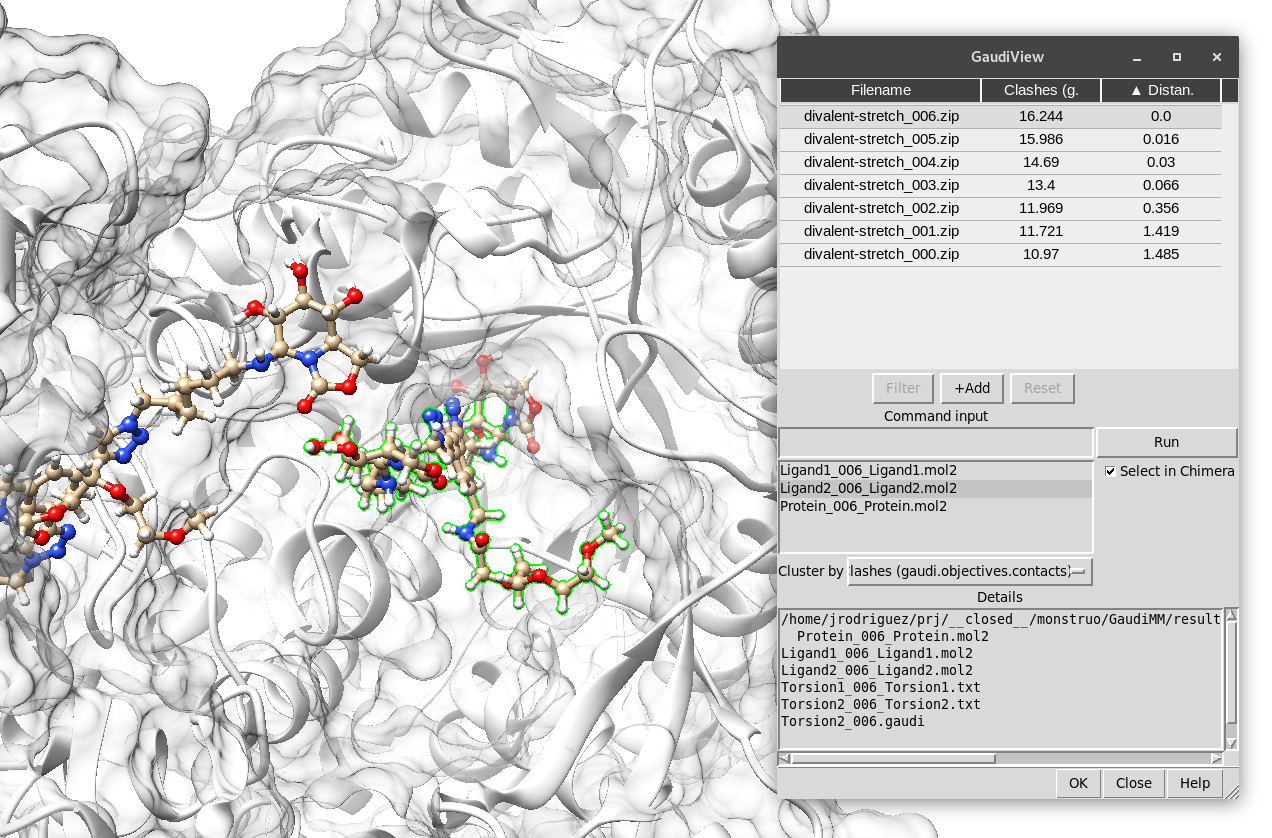
\includegraphics[width=\textwidth]{./figures/04/gaudiview.png}
	\caption[GaudiView]{Analysis of a GaudiMM dual docking calculation with GaudiView. Each row of the table represents one candidate solution that will be depicted in the 3D canvas upon selection.}
	\label{fig:gaudiview}
\end{figure}


\section{The code behind}
% \addcontentsline{toc}{subsection}{The code behind}
GaudiMM was conceived with modularity and extensibility in mind. Stemming from quick drafts on UCSF Chimera's Python interpreter, the codebase rapidly outgrew a single file of a hundred lines into a full-fledged library with thousands of lines of code. Using Python as the main language allowed to design a modular architecture focused on the reutilization of existing codebases easily looking forward obtaining a working proof-of-concept in very little time. All the code is object-oriented, alleviating the process of writing new genes and objectives.

However, UCSF Chimera is still the main library behind the scenes. In fact, to our knowledge, GaudiMM is one of the few projects that relies on it for calculation purposes and not strictly for visualization. This interactive 3D viewer offers lots of analysis tools and robust molecular abstractions that allowed us to implement most of GaudiMM genes and objectives in few lines of code. However, everything has a price and UCSF Chimera was not designed to be used as a library in other projects; instead it expects external projects to be executed within UCSF Chimera interface. To overcome this limitation, a separate package named PyChimera was developed. With PyChimera, other Python libraries can be used together with UCSF Chimera which allowed us to intertwin other projects in GaudiMM. That way, MM energies can be computed with OpenMM, Normal Modes Analysis calculated with ProDy, and more (see tables \ref{table:gaudi-genes} and \ref{table:gaudi-objectives}). Further details are given in \autoref{chap:05}, where PyChimera has proved to also be instrumental in the development and distribution of new graphical interfaces.


\section{Conclusions $\&$  Further work}
% \addcontentsline{toc}{section}{Conclusions $\&$  Further work}
The development of GaudiMM was motivated by the need of applying simple descriptors in complex biomolecular systems featuring residues beyond the natural amino acids: metallic cofactors, oligosugar-derivatives and partially characterized organic molecules. The main idea was to at least have ‘some’ results around a hard-to-model structure, instead of saying that it could not be done. Even with low accuracy methods, GaudiMM soon started to prove that the approach is good enough to provide starting points valid for further refinement and processing with more accurate methods. In other words, GaudiMM is a good entry point for multiscale protocols, which is further discussed in \autoref{chap:05}. Examples of its potential applications and how it has been used in real research will be detailed in \autoref{chap:06}.

When the collection of genes and objectives began to grow, it became unmanageable as a single file script, and a modular object-oriented architecture was devised to hold each descriptor as a separate, but compatible, pieces of code. Using Python as the programming language made this refactoring very easy and allowed implementing new descriptors fast and simply. The educational value of this technical decision was not obvious until degree and master students began to collaborate in the project as part of their final dissertation.

These observations have made clear that GaudiMM provides a mental framework suitable for implementing proof-of-concept multiscale protocols and explaining basic concepts of molecular modeling to newcomers in the field.

That said, there is room for improvement in the performance area. Genetic algorithms are easily parallelizable by design, but depending on UCSF Chimera for most of the functions means that communication across processes could be expensive in terms of memory usage and synchronization overhead. Since the calculations rarely involve more than a few hours, the focus shifted towards the implementation of new modules rather than optimizing the speed of the new ones. However, it is one of the main milestones of the GaudiMM v2.0 roadmap.

\todo[inline]{Further work: dimensionality reduction of the Pareto front for common cases: linearization of multidimensional resutls, new algorithms}